\documentclass[tikz,border=0pt]{standalone}
\usepackage[utf8]{inputenc}
\usepackage[T1]{fontenc}
\usepackage{lmodern}
\usepackage{amsmath,amssymb}
\usetikzlibrary{arrows.meta,positioning,fit,calc,backgrounds,shapes.geometric,decorations.pathreplacing}
\definecolor{navy}{HTML}{163A5F}
\definecolor{blue}{HTML}{2C6EAF}
\definecolor{lightblue}{HTML}{EAF2F8}
\definecolor{midblue}{HTML}{CFE1F2}
\definecolor{graytext}{HTML}{4A5560}
\definecolor{lightgray}{HTML}{F4F6F8}
\definecolor{green}{HTML}{3C8D73}
\definecolor{lightgreen}{HTML}{E8F5EF}
\definecolor{red}{HTML}{B24A4A}
\definecolor{lightred}{HTML}{FBEDEE}
\tikzset{
  title/.style={font=\sffamily\bfseries\fontsize{16}{18}\selectfont,text=navy,anchor=west},
  subtitle/.style={font=\sffamily\bfseries\fontsize{11}{13}\selectfont,text=navy},
  body/.style={font=\sffamily\fontsize{9.2}{11}\selectfont,text=graytext,align=left},
  small/.style={font=\sffamily\fontsize{8}{9.4}\selectfont,text=graytext,align=left},
  tinylabel/.style={font=\sffamily\fontsize{7.2}{8.4}\selectfont,text=graytext},
  panel/.style={rounded corners=3pt,draw=midblue,fill=white,line width=0.6pt},
  box/.style={rounded corners=2pt,draw=midblue,fill=lightblue,line width=0.6pt},
  worker/.style={rounded corners=2pt,draw=blue,dashed,line width=0.7pt,fill=white},
  task/.style={rounded corners=2pt,draw=blue,fill=lightblue,minimum width=0.85cm,minimum height=0.55cm,font=\sffamily\bfseries\small,text=navy},
  file/.style={draw=blue,fill=white,minimum width=0.55cm,minimum height=0.42cm,font=\sffamily\small,text=navy},
  arr/.style={-{Stealth[length=2.4mm,width=1.8mm]},draw=blue,line width=0.9pt},
  arrthin/.style={-{Stealth[length=2mm,width=1.5mm]},draw=blue,line width=0.7pt},
  arrred/.style={-{Stealth[length=2mm,width=1.5mm]},draw=red,dashed,line width=0.8pt},
  arrgreen/.style={-{Stealth[length=2mm,width=1.5mm]},draw=green,dotted,line width=1pt}
}
\begin{document}

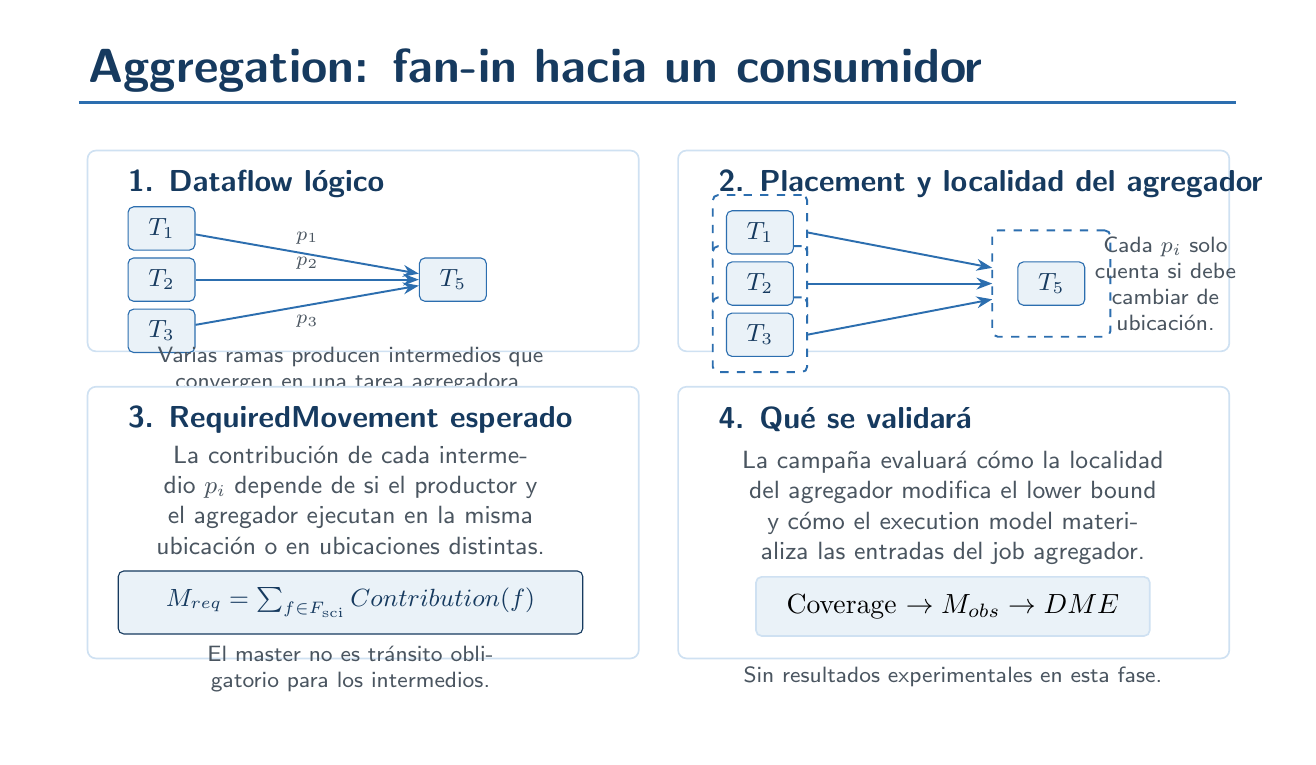
\begin{tikzpicture}[x=1cm,y=1cm]
\path[use as bounding box] (0,0) rectangle (16,9);
\node[title] at (0.65,8.45) {Aggregation: fan-in hacia un consumidor};
\draw[blue,line width=1pt] (0.65,8.05)--(15.35,8.05);
\node[panel,minimum width=7cm,minimum height=2.55cm,anchor=north west] at (0.75,7.45) {};
\node[subtitle,anchor=west] at (1.15,7.02) {1. Dataflow lógico};
\node[task] (t1) at (1.7,6.45) {$T_1$}; \node[task] (t2) at (1.7,5.8) {$T_2$}; \node[task] (t3) at (1.7,5.15) {$T_3$}; \node[task] (t5) at (5.4,5.8) {$T_5$};
\draw[arrthin] (t1)-- node[above,tinylabel] {$p_1$} (t5); \draw[arrthin] (t2)-- node[above,tinylabel] {$p_2$} (t5); \draw[arrthin] (t3)-- node[below,tinylabel] {$p_3$} (t5);
\node[small,text width=5.7cm,align=center] at (4.1,4.65) {Varias ramas producen intermedios que convergen en una tarea agregadora.};
\node[panel,minimum width=7cm,minimum height=2.55cm,anchor=north west] at (8.25,7.45) {};
\node[subtitle,anchor=west] at (8.65,7.02) {2. Placement y localidad del agregador};
\node[worker,minimum width=1.2cm,minimum height=0.95cm] at (9.3,6.4) {}; \node[worker,minimum width=1.2cm,minimum height=0.95cm] at (9.3,5.75) {}; \node[worker,minimum width=1.2cm,minimum height=0.95cm] at (9.3,5.1) {}; \node[worker,minimum width=1.5cm,minimum height=1.35cm] at (13.0,5.75) {};
\node[task] at (9.3,6.4) {$T_1$}; \node[task] at (9.3,5.75) {$T_2$}; \node[task] at (9.3,5.1) {$T_3$}; \node[task] at (13.0,5.75) {$T_5$};
\draw[arrthin] (9.9,6.4)--(12.25,5.95); \draw[arrthin] (9.9,5.75)--(12.25,5.75); \draw[arrthin] (9.9,5.1)--(12.25,5.55);
\node[small,text width=2.0cm,align=center] at (14.45,5.75) {Cada $p_i$ solo cuenta si debe cambiar de ubicación.};
\node[panel,minimum width=7cm,minimum height=3.45cm,anchor=north west] at (0.75,4.45) {};
\node[subtitle,anchor=west] at (1.15,4.02) {3. RequiredMovement esperado};
\node[body,text width=5.8cm,align=center] at (4.1,3.0) {La contribución de cada intermedio $p_i$ depende de si el productor y el agregador ejecutan en la misma ubicación o en ubicaciones distintas.};
\node[rounded corners=2pt,draw=navy,fill=lightblue,minimum width=5.9cm,minimum height=0.8cm,font=\sffamily\bfseries\small,text=navy] at (4.1,1.7) {$M_{req}=\sum_{f\in F_{\mathrm{sci}}} Contribution(f)$};
\node[small,text width=5.7cm,align=center] at (4.1,0.85) {El master no es tránsito obligatorio para los intermedios.};
\node[panel,minimum width=7cm,minimum height=3.45cm,anchor=north west] at (8.25,4.45) {};
\node[subtitle,anchor=west] at (8.65,4.02) {4. Qué se validará};
\node[body,text width=5.7cm,align=center] at (11.75,2.9) {La campaña evaluará cómo la localidad del agregador modifica el lower bound y cómo el execution model materializa las entradas del job agregador.};
\node[box,minimum width=5.0cm,minimum height=0.75cm] at (11.75,1.65) {Coverage $\rightarrow M_{obs} \rightarrow DME$};
\node[small,text width=5.7cm,align=center] at (11.75,0.75) {Sin resultados experimentales en esta fase.};
\end{tikzpicture}
\end{document}
